\documentclass[12pt]{article}
\usepackage[T1]{fontenc}
\usepackage{fullpage,graphicx,psfrag,amsmath,amsfonts}
\usepackage[small,bf]{caption}
\usepackage[utf8]{inputenc}
\usepackage[english]{babel}
\usepackage{lipsum}
\usepackage{url}
\usepackage{bm}
\usepackage{float}
\usepackage{physics}
\usepackage{mathpazo}
\usepackage[12pt]{extsizes}
\usepackage{enumitem}
\usepackage[left=25mm, right=25mm]{geometry}
\newtheorem{theorem}{Theorem}

\begin{document}
\begin{center}
    \vspace*{1cm}    
    \textbf{\LARGE Minimal Autocalibration Pipeline}

    \vspace{0.5cm}
    A minimal approach and experiments
            
    \vspace{1.5cm}

    \textbf{Filippo Grotto VR460638 \\ Matteo Meneghetti VR469054}

    \vspace{0.5cm}
    Master degree in Computer Engineering for Robotics and Smart Industry

    \vfill
            
    Computer Vision 2021/2022
            
    \vspace{0.8cm}
                
    Department of Computer Science\\
    University of Verona\\
            
\end{center}

\tableofcontents

\newpage
\section{Problem Statement}
The main idea of this project is to present a minimal pipeline to estimate intrinsic camera parameters using auto-calibration methods We will assume known corresponding points and an initial estimation of the intrinsic camera parameters. The entire pipeline is based on the dataset provided by Zephyr, in particular, we used 3DFlow Dante dataset.

\section{Pipeline}
\subsection{Data Structure}
Prepare the data structure from the Zephyr dataset. Build a node for each pair of images i, j with the related 3D point and $(uv,vv)$ in the images called correspondence points. Moreover the related rotations $R$, translations $t$ and the original intrinsic parameters $k$ are collected. In this way a symmetric cell $S\{i,j\}$ can be constructed. An example is reported:
\begin{verbatim}
           points: [2147×3 double]
           uv_i: [2147×1 double]
           vv_i: [2147×1 double]
           uv_j: [2147×1 double]
           vv_j: [2147×1 double]
           name_view_i: '_SAM1001.JPG'
           name_view_j: '_SAM1002.JPG'
           K_i: [3×3 double]
           R_i: [3×3 double]
           t_i: [3×1 double]
           K_j: [3×3 double]
           R_j: [3×3 double]
           t_j: [3×1 double]
\end{verbatim}
Finally, \text{name\_view\_i} and \text{name\_view\_j} are the filenames of the related images in case it is necessary.

\subsection{Fundamental Matrices}
Using the corresponding points of a pair of images it is possible to estimate the fundamental matrices. In order to make this estimation as robust as possible RANSAC is executed to extract only inliners. Finally the epipolar lines are calculated to evaluate the fundamental matrix computed. In Fig \ref{fig:epipolar} and \ref{fig:epipolar2} some examples are reported.
\begin{figure}[H]
    \centering
    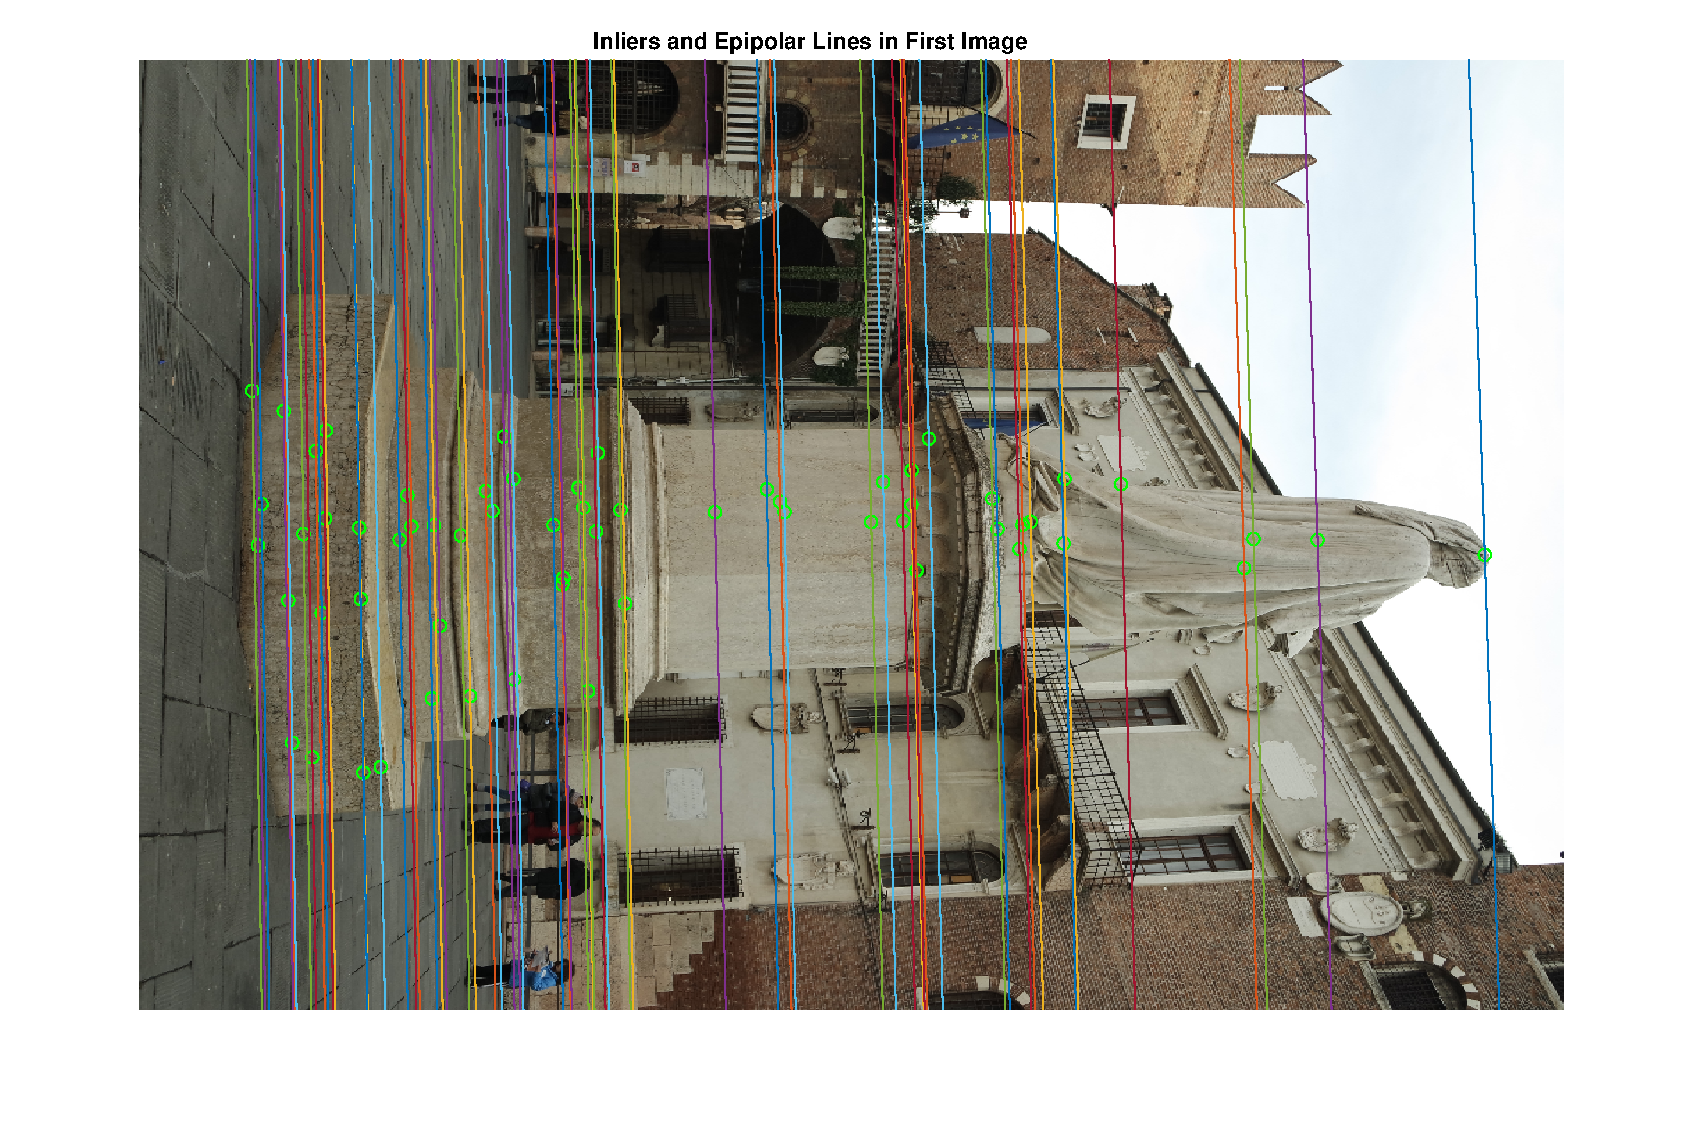
\includegraphics[scale=0.5]{images/epipolar.eps}
    \qquad
    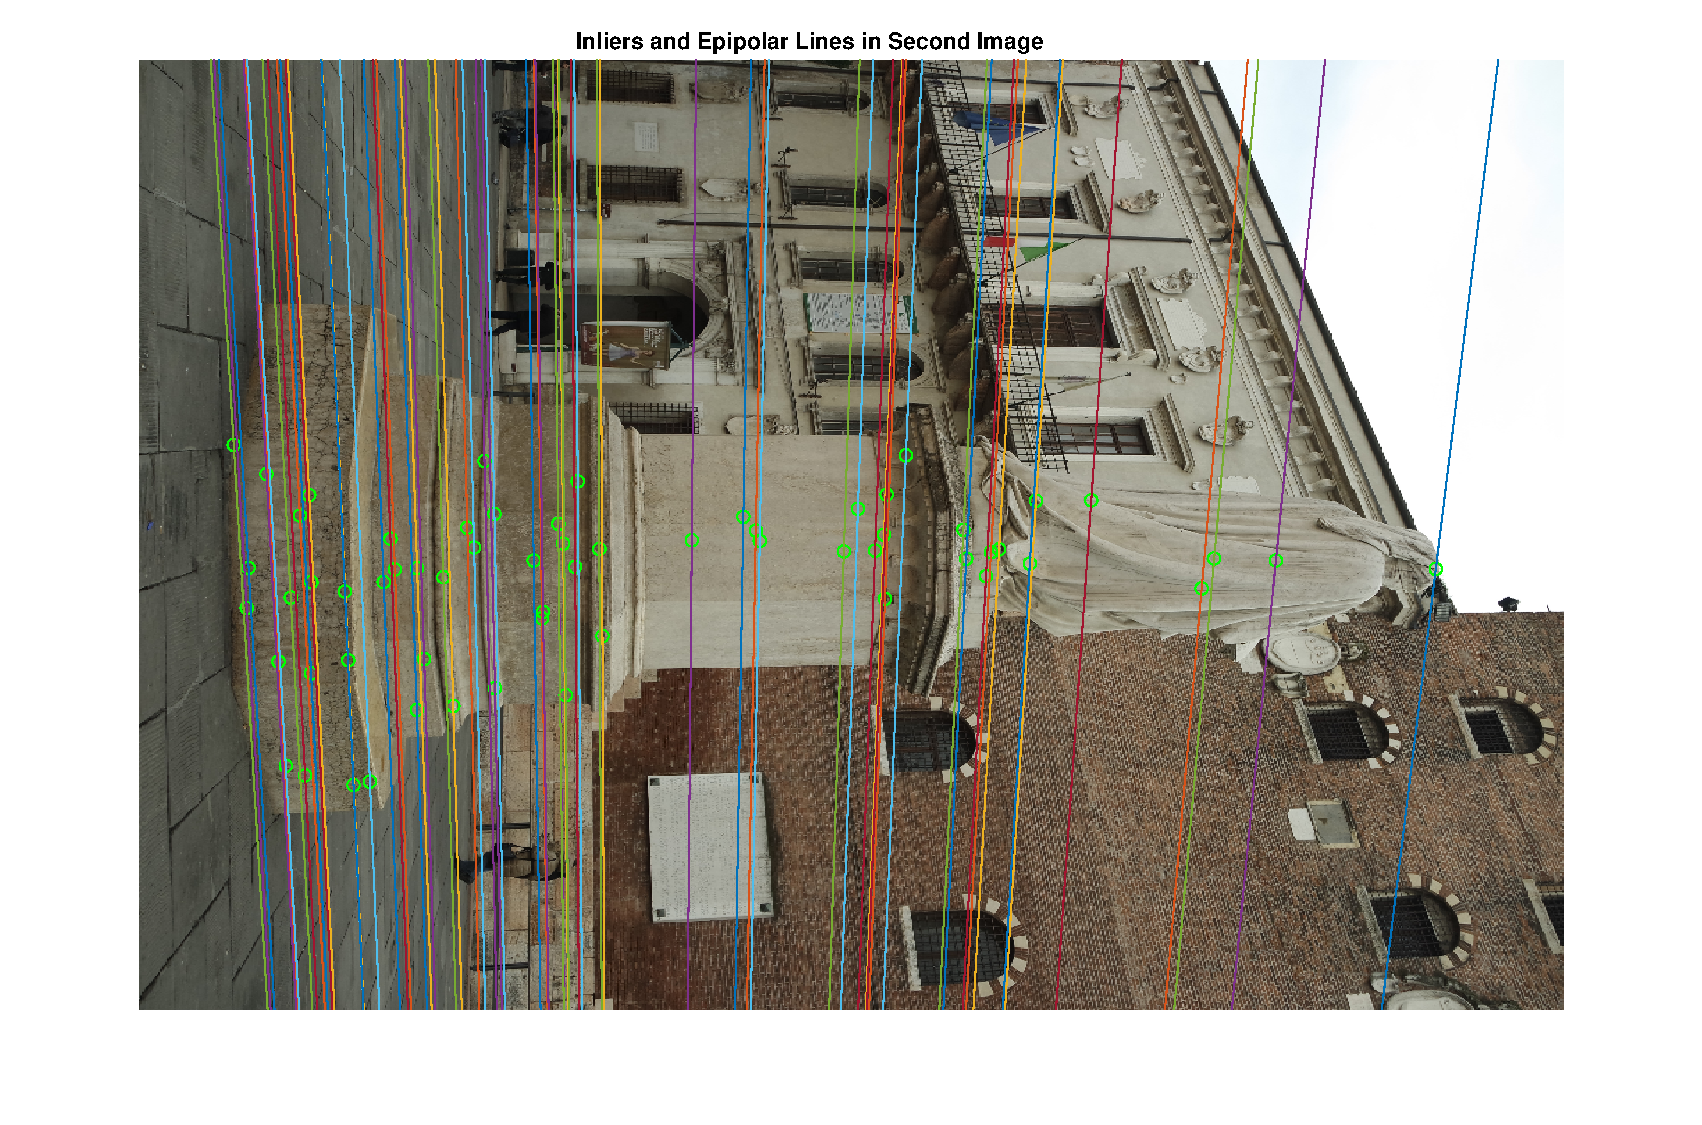
\includegraphics[scale=0.5]{images/epipolar2.eps}
    \caption{Epipolar lines of pair of images 1 and 2 considering the inliers obtained with the RANSAC}
    \label{fig:epipolar}
\end{figure}

\begin{figure}[H]
    \hspace*{-11cm}
    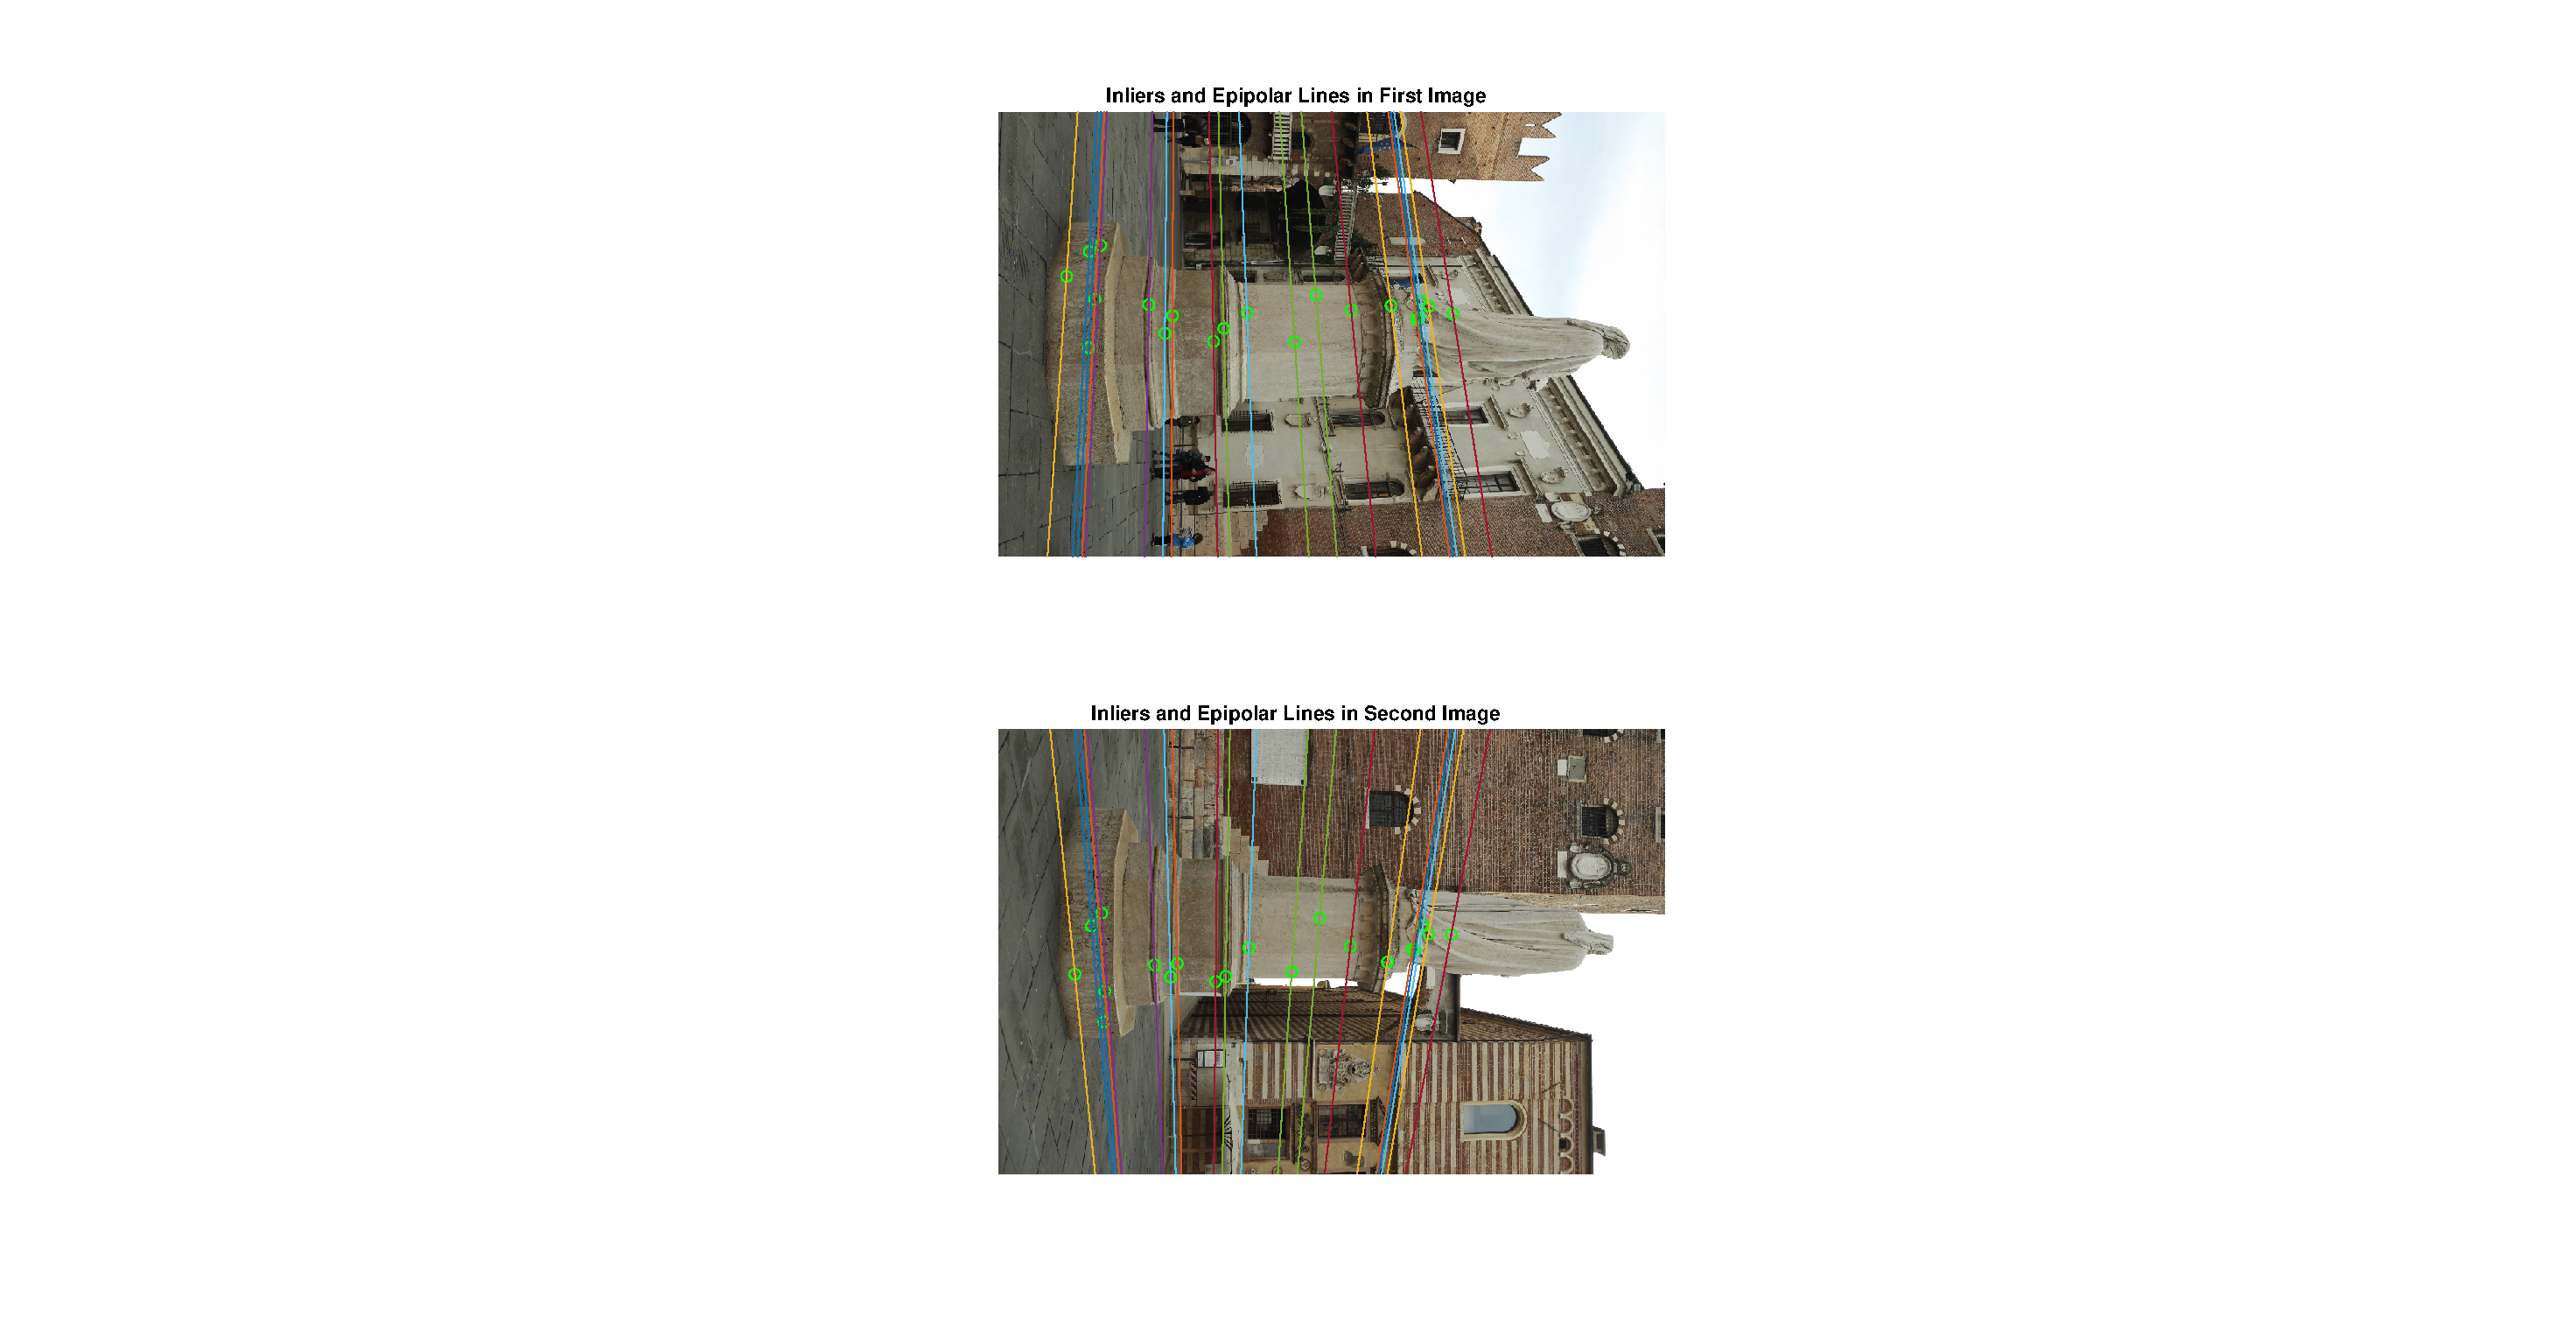
\includegraphics[scale=0.75]{images/epipolar3.eps}
    \caption{Epipolar lines of pair of images considering the inliers obtained with the RANSAC}
    \label{fig:epipolar2}
\end{figure}


\subsection{Autocalibration}
Given the fundamental matrices the autocalibration algorithms require an initial estimation of the matrix $K_0$ of internal camera parameters. To do so a simple script provided in \textbf{compute\_k0.m} was used which extract the intrinsic camera parameters from the size of the image assuming a $35$mm focal length. An example of initial estimation is reported:
\begin{verbatim}
    Initial estimation K0
   1.0e+03 *

    5.9410         0    2.7360
         0    5.9410    1.8240
         0         0    0.0010
\end{verbatim}
which is very close to the original values computed in Zephyr:
\begin{verbatim}
    Original K
    1.0e+03 *
 
     5.7942         0    2.7923
          0    5.7942    1.8174
          0         0    0.0010
\end{verbatim}
\subsubsection{Medonca-Cipolla autocalibration}
The first calibration method is proposed by Medonca and Cipolla in \cite{Medonca99}. Considering the intrinsic parameters parametrized as
\begin{equation}
    K = \begin{bmatrix}
        \alpha_x & s & u_0 \\
        0   & \epsilon\alpha_x & v_0 \\
        0 & 0 & 1
    \end{bmatrix}
\end{equation}
where $\alpha_x$ is the product of the focal length and the magnification factor, $\begin{bmatrix}
    u_0 & v_0
\end{bmatrix}^T$ are the coordinates of the principal point, $s$ is the skew and $\epsilon$ is the aspect ratio.

The main idea is to consider the following cost function for $n$ images:
\begin{equation}
    C(K_i, i = 1,\dots, n) = \sum_{ij}^{n} \frac{w_{ij} (\sigma_{1ij}-\sigma_{2ij})}{\sum_{kl}^{n}w_{kl} \sigma_{2ij}}
\end{equation}
where $\sigma_{1ij}$ and $\sigma_{1ij}$ are the non zero singular values of $K_j^TF_{ij}K_j$ in descending order, considering the fundamental matrix between two images i, j as $F_{ij}$ and the intrinsic parameters $K_j$. The weights $w_{ij}$ are the degree of confidence in the estimation of the fundamental matrix and can be equal to the number of points used in the computation of the fundamental matrix.

\bigskip
The implementation of this method is provided in \textbf{cost\_medonca\_cipolla.m} and can be used with $lsqnonlin$ or $fmincon$ to solve the related minimization problem. Several parameters has been tested but using the computed fundamental matrices and initial estimation the solver (interior point method) simply confirm the presence of a minimal point as:
\begin{verbatim}
    Medonca cipolla: 
    1.0e+03 *
 
     5.9410    0.0000    2.7360
          0    5.9410    1.8240
          0         0    0.0010
 
 Autocalibration % error:	 2.5334  
\end{verbatim}
\subsubsection{Kruppa method autocalibration}
The second calibration method proposed is Kruppa method that can be found in \cite{Prapitasari14}. From the classical Kruppa's equations and cost function can be derived to be solved as a nonlinear least-squares optimization problem:
\begin{equation}
    C = \sum_{ij} ||\frac{F_{ij}w^{-1}F_{ij}^T}{||F_{ij}w^{-1}F_{ij}^T||} - \frac{[e_{ji}]_xw^{-1}[e_{ji}]^T}{||[e_{ji}]_xw^{-1}[e_{ji}]^T||}||
\end{equation}
where $F_{ij}$ are the fundamental matrices, $e$ are the epipoles and $w^{-1} = KK^T$. The norms used are the frobenius norms.

\bigskip
The implementation of this method is provided in \textbf{cost\_kruppas\_method.m} and can be used with $lsqnonlin$ or $fmincon$ to solve the related minimization problem. Several parameters has been tested but using the computed fundamental matrices and initial estimation the solver (interior point method) simply confirm the presence of a minimal point as:
\begin{verbatim}
    Kruppas method: 
    1.0e+03 *
 
     5.9410         0    2.7360
          0    5.9410    1.8240
          0         0    0.0010
 
 Autocalibration % error:	 2.5334   
\end{verbatim}
\subsubsection{Medonca-Cipolla Toolbox}
The last calibration method is provided in the Computer Vision Toolbox from Andrea Fusiello. The main idea is the following theorem from Huang and Faugeras \cite{Faugeras89}
\begin{equation}
    det(E) = 0 \qquad tr((EE^T))^2 - 2 tr((EE^T)^2) = 0
\end{equation}
The previous equation is a condition to have one singular value equal to zero for $E$ and two identical non-zero singular values. This condition can be used to build a cost function like:
\begin{equation}
    C(K) = \sum_{i=1}^{n} \sum_{j=i+1}^{n} w_{ij} (tr((EE^T))^2 - 2 tr((EE^T)^2))ì2
\end{equation}
where $E_{ij} = K'F_{ij}K$ and $w_ij$ are the degree of confidence in the estimation of the fundamental matrix. The cost function is minimized with the matlab algorithms like the previous algorithms but the convergence is not guaranteed for each initial value. An example obtained with this procedure is reported:
\begin{verbatim}
    Medonca cipolla (Toolbox): 
    1.0e+03 *
 
     5.9272         0    2.7360
          0    5.9272    1.8240
          0         0    0.0010
 
 Autocalibration % error:	 2.2954  
\end{verbatim}
\newpage

\subsubsection{Autocalibration considerations}
As it is visible the auto-calibration algorithms improve minimally the initial estimation. The initial estimation is changed only in the medonca-cipolla from the toolbox which reported a small improvement. However this depends on the execution of the RANSAC which is no-deterministic and can change on each execution. Moreover the fundamental matrices play a big role on this estimation,. Frequently the algorithms drop the accuracy to $20-30\%$ of error compared to the initial estimation of $K$. As example using the correct fundamental matrices directly from Zephyr produces in general better and more stable results with around $2\%$ of error. 

\section{Relative orientation and 3D points evaluation}
Finally the relative orientation for each pair of images $(i,j)$ is recovered using the estimated $K$ with the function provided in the computer vision toolbox. The rotation $R_{ji}$ and translation $t_{ji}$ are saved in the related instance $S{i,j}$. Finally the absolute orientation is recovered using the original 3D points and the triangulated 3D points from corresponding points. The orthogonal procrustes problem (opa) is solved to recover the scaling, the rotation and the translation as follow:
\begin{equation}
    D=s(RM+t)
\end{equation}
the actual algorithm is not reported and can be found in th CV toolbox. Another possibility is to concatenate the relative orientation of each view with respect to the first one, triangulate the points and register them with iterative closest point algorithm (icp). However, the latter approach is not as robust as solving opa, it is computationally more expensive and it is not always possible to concatenate close views due to missing common points to compute the fundamental matrices.

\bigskip
In Fig \ref{fig:relative} the results of relative orientations and opa are reported to check the results obtained. In Fig \ref{fig:statue} the final result is reported using the inliers points of 5 views and the estimated $K$.
\begin{figure}[H]
    \centering
    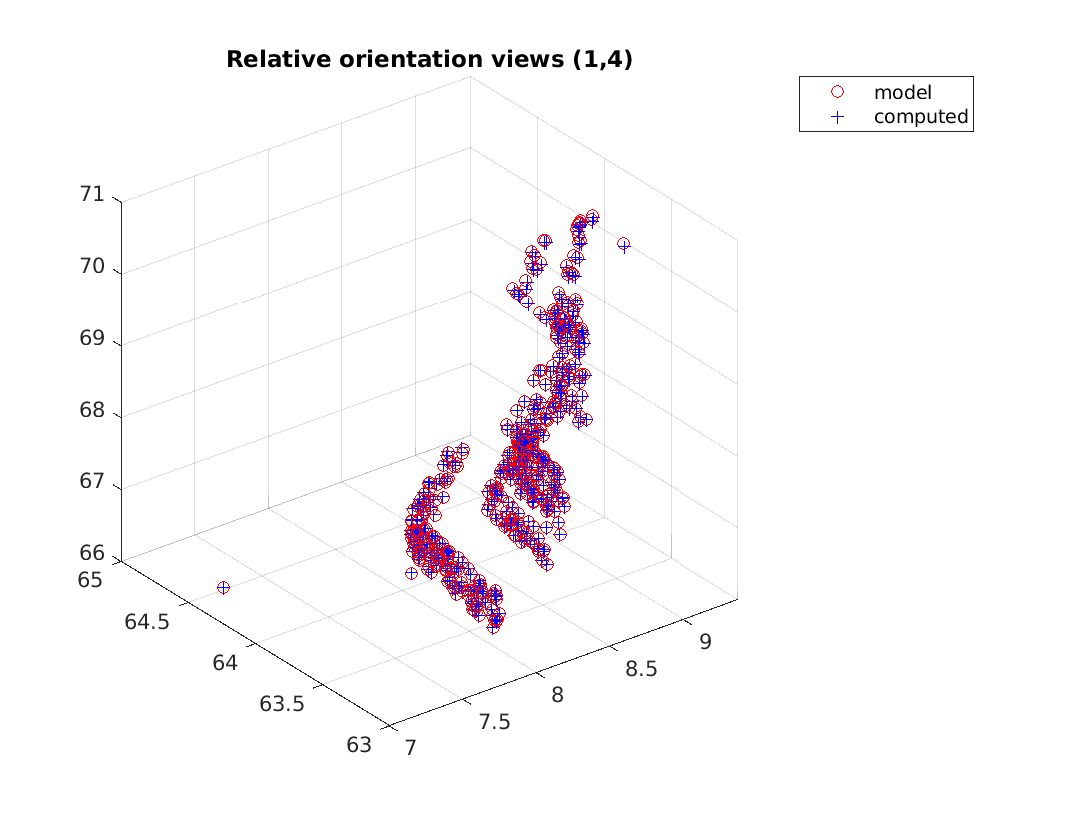
\includegraphics[scale=0.65]{images/relative_3.eps}
    \qquad
    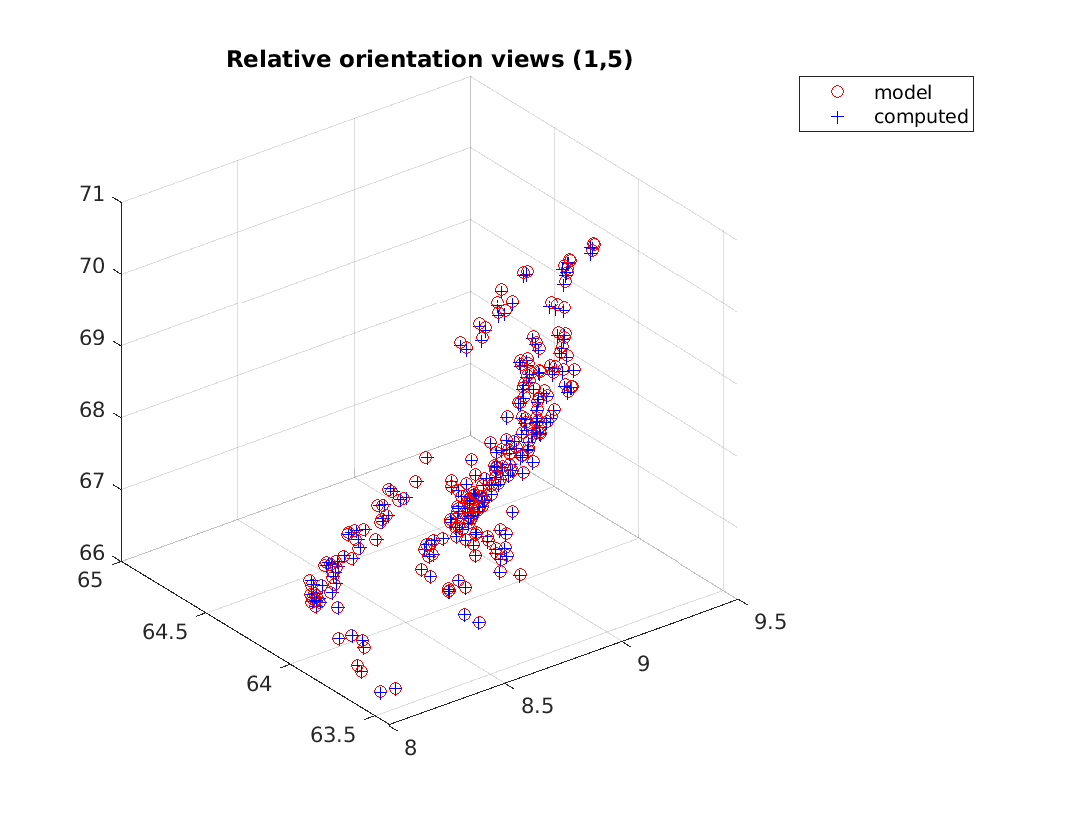
\includegraphics[scale=0.65]{images/relative_4.eps}
    \caption{Example of relative orientations with OPA of the 3D points of the model and the computed ones. Top: relative orientation of images 1 and 4. Bottom: relative orientation of images 2 and 3.}
    \label{fig:relative}
\end{figure}

\begin{figure}[H]
    \centering
    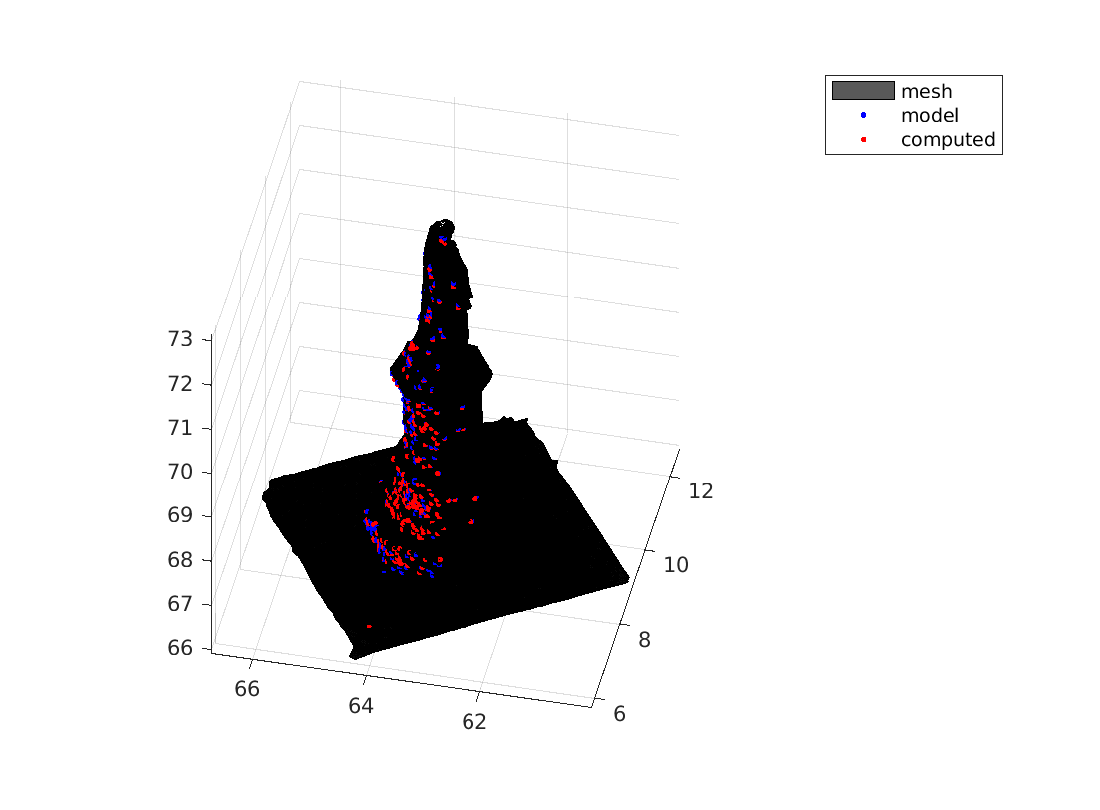
\includegraphics[scale=0.65]{images/statue.eps}
    \caption{Final result using inliers from 5 views}
    \label{fig:statue}
\end{figure}

\section{Final considerations}
This project proposed a minimal pipeline to try auto-calibration algorithms. Three algorithms are presented and the problems related to the correct estimation of the fundamental matrices and the initial estimation has been briefly discussed. It is clear that a good initial estimation is necessary and ad-hoc consideration for the optimizations and the number of fundamental matrices are required. Other more advanced methods can be considered like the one proposed in \cite{Gherardi10} to make the entire process more robust and reliable. 

\newpage
\section{Sample execution of the pipelines}
The file \textbf{pipeline\_dataset.m} will simply save the cell \textbf{S.mat} with the previously explained fields.

\bigskip
\noindent The file \textbf{pipeline\_autocalibration.m} starting from the dataset and the cell previously computed will display the previously discussed images and some logs to show all the steps. An example is reported:
\begin{verbatim}
>> pipeline_autocal
Pipeline for autocalibration starting from S data-structure
Computing fundamental matrices
Fundamental nonlin Smps error views (1, 2):	 0.0031627 
Fundamental nonlin Smps error views (1, 3):	 0.0024425 
Fundamental nonlin Smps error views (1, 4):	 0.002811 
Fundamental nonlin Smps error views (1, 5):	 0.0031565 
Fundamental nonlin Smps error views (1, 6):	 0.0014842 
Fundamental nonlin Smps error views (1, 7):	 0.020671 
Fundamental nonlin Smps error views (2, 1):	 0.0024991 
Fundamental nonlin Smps error views (2, 3):	 0.0030905 
Fundamental nonlin Smps error views (2, 4):	 0.0030361 
Fundamental nonlin Smps error views (2, 5):	 0.0022037 
Fundamental nonlin Smps error views (2, 6):	 0.0026793 
Fundamental nonlin Smps error views (2, 7):	 0.0016929 
Fundamental nonlin Smps error views (3, 1):	 0.0022929 
Fundamental nonlin Smps error views (3, 2):	 0.002401 
Fundamental nonlin Smps error views (3, 4):	 0.0027734 
Fundamental nonlin Smps error views (3, 5):	 0.0024261 
Fundamental nonlin Smps error views (3, 6):	 0.0025424 
Fundamental nonlin Smps error views (3, 7):	 0.014985 
Fundamental nonlin Smps error views (4, 1):	 0.0025035 
Fundamental nonlin Smps error views (4, 2):	 0.0022684 
Fundamental nonlin Smps error views (4, 3):	 0.0026446 
Fundamental nonlin Smps error views (4, 5):	 0.0027064 
Fundamental nonlin Smps error views (4, 6):	 0.0025767 
Fundamental nonlin Smps error views (4, 7):	 0.0021809 
Fundamental nonlin Smps error views (4, 8):	 0.0010518 
Fundamental nonlin Smps error views (4, 9):	 0.0018463 
Fundamental nonlin Smps error views (5, 1):	 0.0020802 
Fundamental nonlin Smps error views (5, 2):	 0.0018484 
Fundamental nonlin Smps error views (5, 3):	 0.0024945 
Fundamental nonlin Smps error views (5, 4):	 0.0024516 
Fundamental nonlin Smps error views (5, 6):	 0.0029323 
Fundamental nonlin Smps error views (5, 7):	 0.0026759 
Fundamental nonlin Smps error views (5, 8):	 0.002029 
Fundamental nonlin Smps error views (5, 9):	 0.0022594 
Fundamental nonlin Smps error views (5, 10):	 0.0019431 
Fundamental nonlin Smps error views (6, 1):	 0.0061476 
Fundamental nonlin Smps error views (6, 2):	 0.0024777 
Fundamental nonlin Smps error views (6, 3):	 0.0027282 
Fundamental nonlin Smps error views (6, 4):	 0.002434 
Fundamental nonlin Smps error views (6, 5):	 0.003016 
Fundamental nonlin Smps error views (6, 7):	 0.0026064 
Fundamental nonlin Smps error views (6, 8):	 0.0019908 
Fundamental nonlin Smps error views (6, 9):	 0.0020711 
Fundamental nonlin Smps error views (6, 10):	 0.0018189 
Fundamental nonlin Smps error views (7, 1):	 0.0031762 
Fundamental nonlin Smps error views (7, 2):	 0.0027499 
Fundamental nonlin Smps error views (7, 3):	 0.00098399 
Fundamental nonlin Smps error views (7, 4):	 0.0021696 
Fundamental nonlin Smps error views (7, 5):	 0.0029434 
Fundamental nonlin Smps error views (7, 6):	 0.0031189 
Fundamental nonlin Smps error views (7, 8):	 0.0024496 
Fundamental nonlin Smps error views (7, 9):	 0.0023762 
Fundamental nonlin Smps error views (7, 10):	 0.0025005 
Fundamental nonlin Smps error views (8, 4):	 0.00084975 
Fundamental nonlin Smps error views (8, 5):	 0.0023448 
Fundamental nonlin Smps error views (8, 6):	 0.0029435 
Fundamental nonlin Smps error views (8, 7):	 0.0029002 
Fundamental nonlin Smps error views (8, 9):	 0.0021972 
Fundamental nonlin Smps error views (8, 10):	 0.0027414 
Fundamental nonlin Smps error views (9, 4):	 0.0031056 
Fundamental nonlin Smps error views (9, 5):	 0.008166 
Fundamental nonlin Smps error views (9, 6):	 0.0024978 
Fundamental nonlin Smps error views (9, 7):	 0.0022805 
Fundamental nonlin Smps error views (9, 8):	 0.0027031 
Fundamental nonlin Smps error views (9, 10):	 0.002577 
Fundamental nonlin Smps error views (10, 5):	 0.00030783 
Fundamental nonlin Smps error views (10, 6):	 0.0020705 
Fundamental nonlin Smps error views (10, 7):	 0.0022292 
Fundamental nonlin Smps error views (10, 8):	 0.0025328 
Fundamental nonlin Smps error views (10, 9):	 0.0028241 
Estimating intrinsic parameters
Original
   1.0e+03 *

    5.7942         0    2.7923
         0    5.7942    1.8174
         0         0    0.0010

Initial estimation
   1.0e+03 *

    5.9410         0    2.7360
         0    5.9410    1.8240
         0         0    0.0010

Medonca cipolla: 
   1.0e+03 *

    5.9410    0.0000    2.7360
         0    5.9410    1.8240
         0         0    0.0010

Autocalibration % error:	 2.5334 

Kruppas method: 
   1.0e+03 *

    5.9410         0    2.7360
         0    5.9410    1.8240
         0         0    0.0010

Autocalibration % error:	 2.5334 

Medonca cipolla (Toolbox): 
   1.0e+03 *

    5.9272         0    2.7360
         0    5.9272    1.8240
         0         0    0.0010

Autocalibration % error:	 2.2954 

Computing relative orientations of views
Relative linear SO3 views (1, 2) error:	 0.014126 
Relative nonlin SO3 views (1, 2) error:	 0.013838 
Relative triang error views (1, 2):	 0.020167 
Relative linear SO3 views (1, 3) error:	 0.016741 
Relative nonlin SO3 views (1, 3) error:	 0.016521 
Relative triang error views (1, 3):	 0.011968 
Relative linear SO3 views (1, 4) error:	 0.029945 
Relative nonlin SO3 views (1, 4) error:	 0.034406 
Relative triang error views (1, 4):	 0.005358 
Relative linear SO3 views (1, 5) error:	 0.026255 
Relative nonlin SO3 views (1, 5) error:	 0.03294 
Relative triang error views (1, 5):	 0.002208 
Relative linear SO3 views (2, 3) error:	 0.010279 
Relative nonlin SO3 views (2, 3) error:	 0.010928 
Relative triang error views (2, 3):	 0.0095837 
Relative linear SO3 views (2, 4) error:	 0.014257 
Relative nonlin SO3 views (2, 4) error:	 0.017974 
Relative triang error views (2, 4):	 0.0053175 
Relative linear SO3 views (2, 5) error:	 0.029462 
Relative nonlin SO3 views (2, 5) error:	 0.029676 
Relative triang error views (2, 5):	 0.0067423 
Relative linear SO3 views (3, 4) error:	 0.011612 
Relative nonlin SO3 views (3, 4) error:	 0.011247 
Relative triang error views (3, 4):	 0.0099209 
Relative linear SO3 views (3, 5) error:	 0.014191 
Relative nonlin SO3 views (3, 5) error:	 0.015126 
Relative triang error views (3, 5):	 0.0032646 
Relative linear SO3 views (4, 5) error:	 0.0092622 
Relative nonlin SO3 views (4, 5) error:	 0.0093469 
Relative triang error views (4, 5):	 0.016286 
Computing final points by view concatenation
Relative triang error views (1, 2):		 0.020167 
Relative triang error views (1, 3):		 0.011968 
Relative triang error views (1, 4):		 0.005358 
Relative triang error views (1, 5):		 0.002208 
Relative triang error views (2, 3):		 0.0095837 
Relative triang error views (2, 4):		 0.0053175 
Relative triang error views (2, 5):		 0.0067423 
Relative triang error views (3, 4):		 0.0099209 
Relative triang error views (3, 5):		 0.0032646 
Relative triang error views (4, 5):		 0.016286 
Pipeline completed
\end{verbatim}

\begin{thebibliography}{100}
    \addtolength{\leftmargin}{0.2in}
    \setlength{\itemindent}{-0.2in}

    \bibitem{Gherardi10} Riccardo Gherardi and Andrea Fusiello "Practical Autocalibration", ECCV10
    \bibitem{Medonca99} Medonca and Cipolla A Simple Technique for Self-Calibration
    \bibitem{Prapitasari14} A Study of Kruppa’s Equation for Camera Self-calibration
    \bibitem{Faugeras89} Huang T. and Faugeras O. Some properties of the E matrix in two-view motion estimation. 
\end{thebibliography}

\end{document}